\documentclass[../../main.tex]{subfiles}
\begin{document}

与えられた数列
\begin{align}
  \begin{cases}
    \displaystyle a_n=\sum_{k=1}^n\dfrac{1}{\sqrt{k}} \\
    \displaystyle b_n=\sum_{k=1}^n\dfrac{1}{\sqrt{2k+1}}
  \end{cases}
\end{align}
について考える．

一般に$0<x$で与えられた単調減少関数$f(x)\, (>0)$について，$\sum_{k=1}^{n}f(k)$は下図の斜線部の短冊部分の合計面積に合致する．

\begin{figure}[htb]
  \centering
  \begin{tikzpicture}[x=1.35cm, y=1.8cm, >=stealth, every node/.style={font=\small}]

    % ============================================================
    % 【左側】下からの評価: \int_1^{n+1} f(x)dx < \sum_{k=1}^n f(k)
    % ============================================================
    \begin{scope}[xshift=0cm]

      % 短冊の塗りつぶし: [k, k+1] で高さ f(k) = 1/sqrt(k)
      % k=1: [1, 2] x [0, 1.0]
      \fill[pattern=north east lines, pattern color=blue!65, opacity=0.7] (1, 0) rectangle (2, 1.0);
      % k=2: [2, 3] x [0, 1/sqrt(2) ≈ 0.707]
      \fill[pattern=north east lines, pattern color=blue!65, opacity=0.7] (2, 0) rectangle (3, 0.7071);
      % k=3: [3, 4] x [0, 1/sqrt(3) ≈ 0.577]
      \fill[pattern=north east lines, pattern color=blue!65, opacity=0.7] (3, 0) rectangle (4, 0.5774);

      % 短冊の輪郭線
      \draw[thick, blue!85!black] (1, 0) rectangle (2, 1.0);
      \draw[thick, blue!85!black] (2, 0) rectangle (3, 0.7071);
      \draw[thick, blue!85!black] (3, 0) rectangle (4, 0.5774);

      % 曲線 y = 1/sqrt(x) の描画 (1 <= x <= 4.3)
      \draw[line width=1.6pt, red!85!black, domain=0.8:4.3, samples=60]
      plot (\x, {1.0/sqrt(\x)});
      \node[red!90!black, font=\footnotesize, above right] at (2.2, 0.8) {$y = f(x)$};

      % 座標軸
      \draw[->, thick, gray!80!black] (-0.2, 0) -- (4.6, 0) node[right] {$x$};
      \draw[->, thick, gray!80!black] (0, -0.2) -- (0, 2.2) node[above] {$y$};
      \node[below left=2pt] at (0, 0) {$O$};

      % 目盛り
      \node[below=2pt, font=\scriptsize] at (1, 0) {$1$};
      \node[below=2pt, font=\scriptsize] at (2, 0) {$2$};
      \node[below=2pt, font=\scriptsize] at (3, 0) {$k$};
      \node[below=2pt, font=\scriptsize] at (4, 0) {$k+1$};

      % 高さのラベル
      \node[left=2pt, font=\tiny, blue!90!black] at (1, 1.0) {$f(1)$};
      \node[left=2pt, font=\tiny, blue!90!black] at (2, 0.7071) {$f(2)$};
      \node[left=2pt, font=\tiny, blue!90!black] at (3, 0.5774) {$f(k)$};
    \end{scope}

    % ============================================================
    % 【右側】上からの評価: \sum_{k=1}^n f(k) < f(1) + \int_1^n f(x)dx
    % ============================================================
    \begin{scope}[xshift=6.0cm]

      % 短冊の塗りつぶし:
      % k=1 の孤立ブロック: [0, 1] x [0, 1] または [1, 2] で高さ f(2)
      % [1, 2] で高さ f(2) ≈ 0.707
      \fill[pattern=north west lines, pattern color=teal!70, opacity=0.7] (1, 0) rectangle (2, 0.7071);
      % [2, 3] で高さ f(3) ≈ 0.577
      \fill[pattern=north west lines, pattern color=teal!70, opacity=0.7] (2, 0) rectangle (3, 0.5774);
      % [3, 4] で高さ f(4) = 0.5
      \fill[pattern=north west lines, pattern color=teal!70, opacity=0.7] (3, 0) rectangle (4, 0.5);

      % 短冊の輪郭線
      \draw[thick, teal!85!black] (1, 0) rectangle (2, 0.7071);
      \draw[thick, teal!85!black] (2, 0) rectangle (3, 0.5774);
      \draw[thick, teal!85!black] (3, 0) rectangle (4, 0.5);

      % 曲線 y = f(x)
      \draw[line width=1.6pt, red!85!black, domain=0.8:4.3, samples=60]
      plot (\x, {1.0/sqrt(\x)});
      \node[red!90!black, font=\footnotesize, above right] at (2.2, 0.8) {$y = f(x)$};

      % 座標軸
      \draw[->, thick, gray!80!black] (-0.2, 0) -- (4.6, 0) node[right] {$x$};
      \draw[->, thick, gray!80!black] (0, -0.2) -- (0, 2.2) node[above] {$y$};
      \node[below left=2pt] at (0, 0) {$O$};

      % 目盛り
      \node[below=2pt, font=\scriptsize] at (1, 0) {$1$};
      \node[below=2pt, font=\scriptsize] at (2, 0) {$2$};
      \node[below=2pt, font=\scriptsize] at (3, 0) {$k-1$};
      \node[below=2pt, font=\scriptsize] at (4, 0) {$k$};

      % 高さのラベル
      \node[right=2pt, font=\tiny, teal!90!black] at (2, 0.7071) {$f(2)$};
      \node[right=2pt, font=\tiny, teal!90!black] at (3, 0.5774) {$f(3)$};
      \node[right=2pt, font=\tiny, teal!90!black] at (4, 0.5) {$f(k)$};
    \end{scope}

  \end{tikzpicture}
  \caption{単調減少関数における短冊の面積と定積分の不等式評価}
  \label{fig:rectangle_integral_comparison}
\end{figure}

% TODO: y=1/sqrt(x)とy=1/sqrt(x+1/2)のグラフ
\begin{figure}[htb]
  \centering
  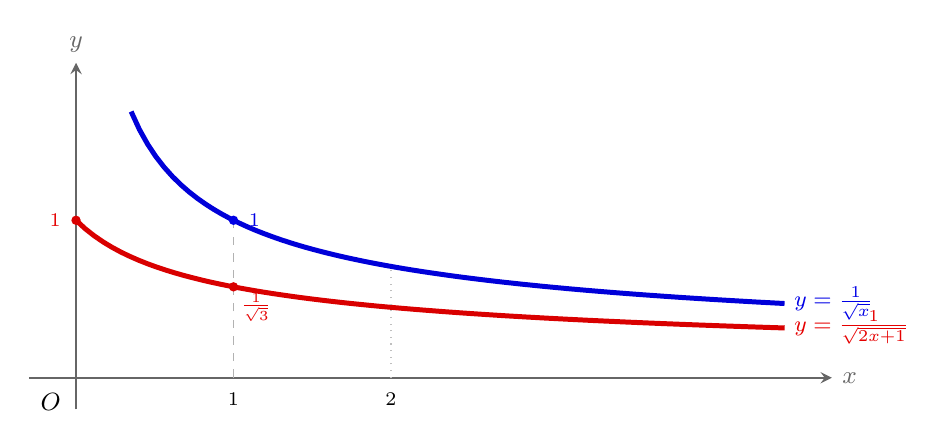
\begin{tikzpicture}[scale=2.0, >=stealth, every node/.style={font=\small}]

    % --- 1. 座標軸 ---
    \draw[->, thick, gray!80!black] (-0.3, 0) -- (4.8, 0) node[right] {$x$};
    \draw[->, thick, gray!80!black] (0, -0.2) -- (0, 2.0) node[above] {$y$};
    \node[below left=2pt] at (0, 0) {$O$};

    % --- 2. 曲線 y = 1/sqrt(x) (青実線) ---
    \draw[line width=1.8pt, blue!85!black, domain=0.35:4.5, samples=80]
    plot (\x, {1.0/sqrt(\x)});
    \node[blue!90!black, font=\footnotesize\bfseries, right] at (4.5, {1.0/sqrt(4.5)})
    {$y = \frac{1}{\sqrt{x}}$};

    % --- 3. 曲線 y = 1/sqrt(2x+1) (赤実線) ---
    \draw[line width=1.8pt, red!85!black, domain=0.0:4.5, samples=80]
    plot (\x, {1.0/sqrt(2.0*\x + 1.0)});
    \node[red!90!black, font=\footnotesize\bfseries, right] at (4.5, {1.0/sqrt(2.0*4.5 + 1.0)})
    {$y = \frac{1}{\sqrt{2x+1}}$};

    % --- 4. x = 0, 1 での切片・代表値と投影破線 ---
    % x = 0 での y = 1/sqrt(2x+1) = 1
    \node[circle, fill=red!85!black, inner sep=1.2pt] at (0, 1.0) {}; \node[left=2pt, font=\scriptsize, red!90!black] at (0, 1.0) {$1$};

    % x = 1 での比較
    % 1/sqrt(1) = 1.0
    % 1/sqrt(3) ≈ 0.577
    \draw[dashed, gray!60] (1.0, 0) -- (1.0, 1.0);
    \node[circle, fill=blue!90!black, inner sep=1.2pt] at (1.0, 1.0) {};
    \node[circle, fill=red!85!black, inner sep=1.2pt] at (1.0, {1.0/sqrt(3.0)}) {};

    \node[below=2pt, font=\scriptsize] at (1.0, 0) {$1$};
    \node[right=2pt, font=\scriptsize, blue!90!black] at (1.0, 1.0) {$1$};
    \node[below right=-1pt, font=\scriptsize, red!90!black] at (1.0, {1.0/sqrt(3.0)}) {$\frac{1}{\sqrt{3}}$};

    % x = 2 での目盛り
    \draw[dotted, gray!50] (2.0, 0) -- (2.0, {1.0/sqrt(2.0)});
    \node[below=2pt, font=\scriptsize] at (2.0, 0) {$2$};

  \end{tikzpicture}
  \caption{$y = \dfrac{1}{\sqrt{x}}$ と $y = \dfrac{1}{\sqrt{2x+1}}$ のグラフ}
  \label{fig:reciprocal_sqrt_functions_comparison}
\end{figure}

従って面積の比較から$a_n,b_n$について，$n$が十分に大きい時，
\begin{align}
  \int_{1}^{n+1}\dfrac{1}{\sqrt{x}}dx < a_n < \int_{1}^{n}\dfrac{1}{\sqrt{x}}dx+1 \label{eq:1}
\end{align}
および
\begin{align}
  \int_{1}^{n+1}\dfrac{1}{\sqrt{2x+1}}dx < b_n < \int_{0}^{n}\dfrac{1}{\sqrt{2x+1}}dx \label{eq:2}
\end{align}
を得る．ただし\cref{eq:1}では$x=0$で$\dfrac{1}{\sqrt{x}}$が発散することに注意した．\cref{eq:1,eq:2}で積分を具体的に計算して
\begin{align}
  \left[2\sqrt{x}\right]_{1}^{n+1} &< a_n < \left[2\sqrt{x}\right]_{1}^{n}+1 \\
  \therefore
  2\sqrt{n+1} - 2 &< a_n < 2\sqrt{n} - 1 \label{eq:3}
\end{align}
および
\begin{align}
  \left[\sqrt{2x+1}\right]_{1}^{n+1} &< b_n < \left[\sqrt{2x+1}\right]_{0}^{n} \\
  \therefore
  \sqrt{2n+3} - \sqrt{3} &< b_n < \sqrt{2n+1} - 1 \label{eq:4}
\end{align}
である．

\paragraph{$\lim_{n\to\infty}a_n$について}

\cref{eq:3}において$n\to\infty$を考えると両辺は正の無限大に発散するから，追い出しの定理から
\begin{align}
  \lim_{n\to\infty}a_n = 0 \cdots\text{(答)}
\end{align}
である．

\paragraph{$\lim_{n\to\infty} \dfrac{b_n}{a_n}$について}

\cref{eq:3,eq:4}において$n\to\infty$を考えるので各辺が正だとしてよく，整理して
\begin{align}
  \dfrac{\sqrt{2n+3} - \sqrt{3}}{2\sqrt{n} - 1} < \dfrac{b_n}{a_n} < \dfrac{\sqrt{2n+1} - 1}{2\sqrt{n+1} - 2} \\
  \dfrac{\sqrt{2+3/n} - \sqrt{3/n}}{2 - 1/\sqrt{n}} < \dfrac{b_n}{a_n} < \dfrac{\sqrt{2+1/\sqrt{n}} - 1/\sqrt{n}}{2\sqrt{1+1/n} - 2/\sqrt{n}}
\end{align}
である．$n\to\infty$の時，両辺ともに$\dfrac{1}{\sqrt{2}}$に収束するから挟み撃ちの定理より
\begin{align}
  \lim_{n\to\infty} \dfrac{b_n}{a_n} = \dfrac{1}{\sqrt{2}} \cdots\text{(答)}
\end{align}
である．

\newpage
\end{document}
